\setcounter{equation}{24}
\setcounter{section}{5}
\setcounter{subsection}{4}
\setcounter{subsubsection}{1}

\paragraph{Erinnerung Erhaltungssätze}~\\
	In Streu-Prozessen gilt die Erhaltung von Energie und Impuls:
	\begin{important}
		\textbf{Energie:}
		\begin{equation}
			\hbar\omega_0 = \hbar\omega\pm\hbar\Omega
		\end{equation}
		\textbf{Impuls:}
		\begin{equation}
			\hbar\vec k_0 = \hbar\vec k\pm\hbar\vec K+\hbar\vec G
		\end{equation}
	\end{important}
	Bei der Lichstreuung kann $\hbar\vec G$ vernachlässigt werden.

\paragraph{Energieverhältnisse für Lichstreuung (sichtbares Licht $\omega$)}~\\
	Optische Photonen haben Frequenzen $\Omega_\mathrm{opt}$ mit  
	$$
		\omega \simeq \SI{100}{\Omega_{\text{opt}}}.
	$$
	Akustische Photonen haben Frequenzen $\Omega_\mathrm{ak}$ mit
	$$
		\omega \simeq (1000\ldots\infty)\,\Omega_\mathrm{ak}.
	$$
	In Streuprozessen ist daher allgemein $\omega\simeq\omega_0$ und $|\vec k|\simeq|\vec k_0|$. 
	Wir betrachten die geometrische Überlegung in \autoref{fig:vl22_abbildung_1}.
	\begin{figure}[H]
		\centering
		\def\svgwidth{.434\columnwidth}
		\subimport{figures/}{vl22_abbildung_1.pdf_tex}
		\caption{Da $|\vec k|\simeq|\vec k_0|$, liegen beide Vektoren auf der Oberfläche eines Kreises. Die Phononen haben dann die Wellenzahl $\vec k_\mathrm{Phonon}$ (rot).}
		\label{fig:vl22_abbildung_1}
	\end{figure}
	Somit ist
	$$
		|\Vec{k}|_{\text{Phonon}} = 2 |\Vec{k}| \sin\left( \frac{\varphi}{2} \right)
	$$
	und
	$$
		\lambda_{\text{Photon}} = 2 \lambda_{\text{Phonon}} \sin\left( \frac\varphi2 \right)
	$$ 

	In Prozessen der Vorwärtsstreuung ist $\varphi=0$ und somit
	$$
		|\Vec{k}_{\text{Phonon}}| = 2 |\Vec{k}| \sin\left( \varphi /2 \right) =0
	$$
	Bei der Rückwärtsstreuung ist $\varphi=\pi$, also
	$$|\Vec{k}_{\text{Phonon}}| = 2 |\Vec{k}|.$$
	Die Wellenzahl der Phononen ist also begrenzt durch
	$$
		0 \le | \Vec{k}_{\text{Phonon}}| \le 2 |\Vec{k}_{\text{Photon}}|
	$$ 
	Bei der Streuung von sichtbarem Licht $\lambda = \SI{500}{nm}$ liegt die Wellenzahl somit in der Größenordnung
	$$
		k = \frac{2\pi}{\lambda} = \frac{2\pi}{\SI{5000}{\angstrom}} \approx \frac{\pi}{1000a}
	$$
	mit der Gitterkonstante von Kristallen $a$. Der größtmögliche Phononenwellenvektoren ist jedoch $k=\frac\pi a$. Die Wechselwirkung mit Licht findet daher nur bei $k\approx0$ statt.
	$$
		|k_\mathrm{max}|=\frac\pi a.
	$$
	\begin{figure}[H]
		\centering
		\incfig{vl22_abbildung_2}
		\caption{Dispersionsrelation für Phononen und die $k$-Bereiche der Wechselwirkung mit Licht.}
		\label{fig:vl22_abbildung_2}
	\end{figure}

	Man unterscheidet 3 Streuprozesse:
	\begin{enumerate}
		\item Ramanstreuung mit $\omega_{\text{L}} \pm \Omega_{\text{opt}}$ 
		\item Brillouinstreuung mit $\omega_{\text{L}} \pm \Omega_{\text{akust}}$ 
		\item Rayleigh-Streuung mit $\omega_{\text{L}}$
	\end{enumerate}

\paragraph{Versuchsanordnung (schematisch)}\,\\
	\begin{figure}[H]
		\centering
		\incfig{vl22_abbildung_3}
		\caption{Schematische Versuchsanordnung für die Phononenspektroskopie.}
		\label{fig:vl22_abbildung_3}
	\end{figure}
	Es gilt $\Delta \omega = \Omega$ unabhängig von der Laserfrequenz. Die Wellenzahlen sind begrenzt durch
	$$
	\Omega < \omega_{\text{L}} < \omega_{m,n}
	$$ 
	mit der Energie $\omega_{m,n}$ von elektronischen Zuständen im Festkörper.

\paragraph{Schematisches Spektrum}\,\\ 
	\begin{figure}[H]
		\centering
		\incfig{vl22_abbildung_4}
		\caption{Schematisches Spektrum der Phononenspektroskopie mit Licht.}
		\label{fig:vl22_abbildung_4}
	\end{figure}
	\begin{verbal}
		Die Linien tauchen allgemein in Dreierpaaren auf.
		Grund dafür sind die drei Raumachsen, entlang derer Phononen sich ausbreiten können (1x longitudinal, 2x transversal).
	\end{verbal}

\paragraph{Energieniveau-Schema}\,\\ 
	\begin{figure}[H]
		\centering
		\incfig{vl22_abbildung_5}
		\caption{Schematisches Energieniveauschema mit Streuprozessen (Stokes, Anti-Stokes) der Phononenspektroskopie.\\
			$u_{l,m,n}$ sind reale stationäre Zustände des Systems.\\
			VZ bezeichnen virtuelle Zwischenzustände.
		}
		\label{fig:vl22_abbildung_5}
	\end{figure}
	\begin{verbal}
		Das Energieschema erklärt in \autoref{fig:vl22_abbildung_4} die höheren Intensitäten beim Stokes-Prozess als beim Anti-Stokes.
		Um Anti-Stokes zu beobachten, muss der Phononenzustand schon besetzt sein.
		DIe Besetzung der Phononenzustände folgt einer Boltzmann-Verteilung.
		Deswegen laufen im Durchschnitt mehr Stokes- als Antistokes-Prozesse ab.
	\end{verbal}
	In \autoref{fig:vl22_germanium} bis \ref{fig:vl22_Indiumantimonid} werden mit Licht gemessene Phononenspektren gezeigt und deren Eigenschaften erklärt. 
	\begin{figure}[H]
		\centering
		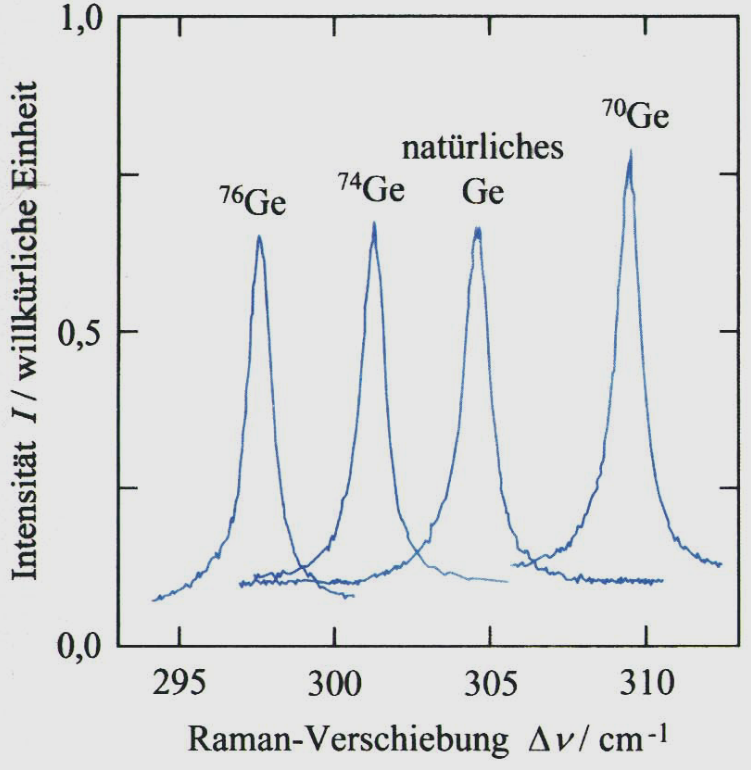
\includegraphics[width=0.5\linewidth]{figures/vl22/germanium.png}
		\caption{Ramanspektrum von Germanium \cite{Hunklinger}. 
			Germaium besitzt eine zweiatomige Basis, jedoch mit nur einer Atomsorte.
			Deshalb ist $\Omega_\mathrm{LO}=\Omega_\mathrm{TO}$ bei $k=0$.
			Deshalb ist nur eine Linie pro Isotop sichtbar.
			So kann die Isotopenreinheit untersucht werden.
		}
		\label{fig:vl22_germanium}
	\end{figure}
	\begin{figure}[H]
		\centering
		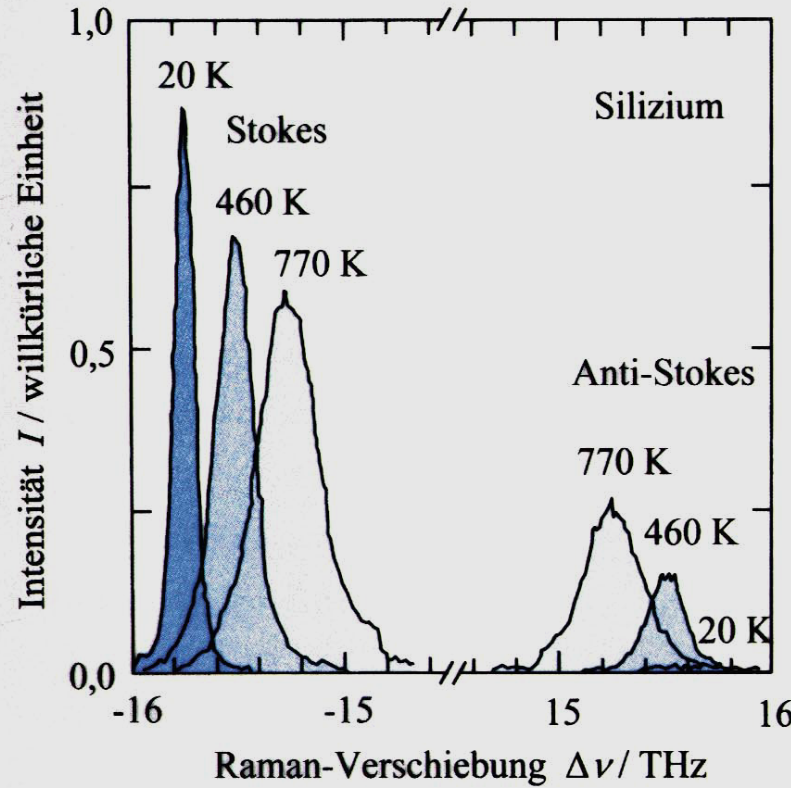
\includegraphics[width=0.5\linewidth]{figures/vl22/silizium.png}
		\caption{Temperaturabhängiges Ramanspektrum von Silizium \cite{Hunklinger}. 
			Mit zunehmender Temperatur beobachtet man eine Zunahme des Intensitätsverhältnisses $I_\mathrm{Anti-Stokes}/I_\mathrm{Stokes}$.
			Dies liegt an der zunehmenden Besetzung höherer Phononenzustände mit zunehmender Temperatur.
			Die Linien rücken mit zunehmender Temperatur ebenfalls weiter zusammen und die Linienbreite nimmt zu. Dies liegt an der Anharmonizität des Gitters.
		}
		\label{fig:vl22_silizium}
	\end{figure}
	\begin{figure}[H]
		\centering
		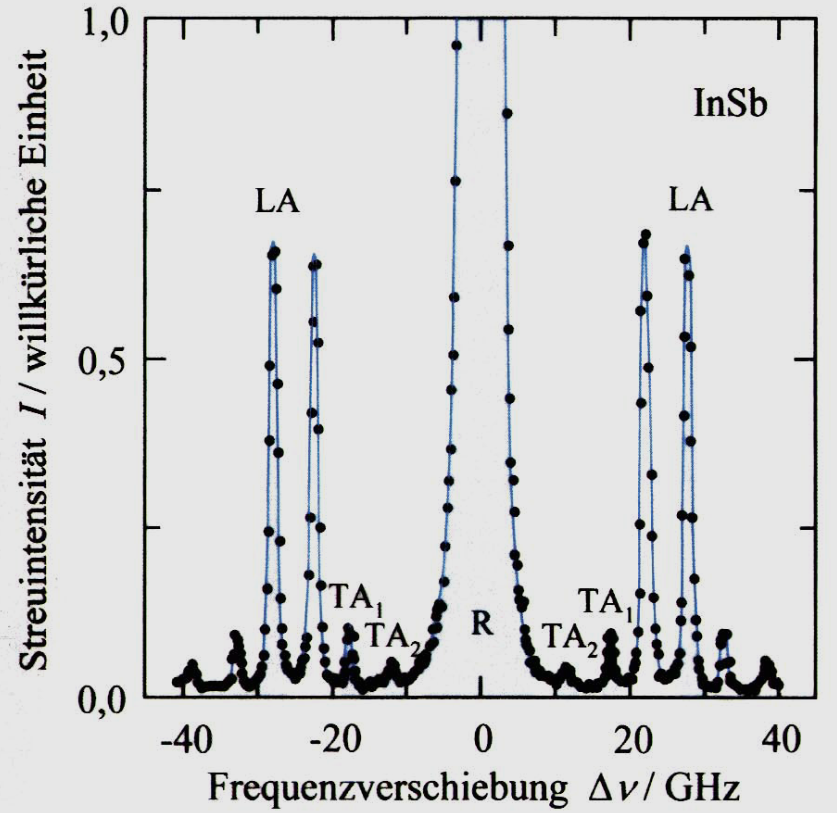
\includegraphics[width=0.5\linewidth]{figures/vl22/indium.png}
		\caption{Brillouinspektrum von Indiumantimonid \cite{Hunklinger}. 
			Wegen seiner zweiatomigen Basis hat Indiumantimonid sowohl im Stokes- als auch im Anti-Stokes-Spektrum je drei Spektrallinien (blau).
			Zusätzliche sichtbare Linien werden durch höhere Ordnungen verursacht (Fabry-Perot-Spektrometer).
		}B von Indiumanti
		\label{fig:vl22_Indiumantimonid}
	\end{figure}
	\paragraph{Anforderungen an die Apparaturen}
	\begin{itemize}
		\item Laseranregung ist optimal. Notwendige Eigenschaften des Lasers sind:
			\begin{enumerate}
				\item hohe Intensitäten
				\item monochromatisch
				\item Bündelung	
			\end{enumerate}
		\item Es wird ein Doppelmonochromator zur Streulichtunterdrückung (Raman) benötigt.
		\item Bei der Brillouinstreuung wird ein Fabry-Pérot-Interferometer benötigt.
			So kann eine hohe Auflösung realisiert werden ($\SI{0.1}{\centi\meter^{-1}}$ bei $\SI{20000}{\centi \meter^{-1}}$, $A = \num{200000}$)
		\item ccd-Kameras werden zur Photonenzählung verwendet (APD, Photomultiplier).
		\item Die Polarisation muss beachtet werden: Raman-Spektren von Festkörpern sind polarisiert und hängen von der Orientierung des Kristalls ab.
	\end{itemize}

\paragraph{Ultrarotspektroskopie}\,\\ 
	Die Ultrarotspektroskopie ist ein direkter Prozess mit $\omega = \Omega$ und $\Vec{k} = \Vec{K}$.

	{Beispiel (\ce{NaCl}):}\\
	Natriumchlorid hat die stärkste IR-Absorption bei $\lambda_{\text{vak}} = \SI{61}{\micro \meter}$.
	Die Wellenzahl der Photonen ist also 
	$$k = 2\pi/\lambda = \SI{e3}{\centi \meter ^{-1}}$$
	Die maximale Wellenzahl der Phononen beträgt 
	$$K_{\text{max}} = \pi / a = \SI{0,55e8}{\centi \meter ^{-1}}.$$
	Die Wellenzahl von Infrarotstrahlung beträgt jedoch
	$$k_{\text{ir}} = \SI{2e-5}{\pi \per a}!$$
	IR-Photonen können also nur transversale optische Phononen (TO) bei $K=0$ anregen.

\subsubsection{Neutronenstreuung}
	Thermische Neutronen sind für die inelastische Streuung an Phononen bestens geeignet. 
	Die Größenordnung solcher Neutronen liegt
	\begin{itemize}
		\item für die Energie bei $E = \SI{1}{\milli \electronvolt}$ bis \SI{100}{\milli \electronvolt} und
		\item für die Wellenzahl bei $|\Vec{k}| = \SI{e7}{\centi \meter ^{-1}}$ bis $\SI{e8}{\centi \meter ^{-1}}$.
	\end{itemize}
	Dadurch können thermische Neutronen mit allen Phononen wechselwirken.

\paragraph{Erhaltungssätze}~\\
 Die Energie ist bei der Neutronenstreuung erhalten:
	\begin{important}
		$$
		\frac{\hbar ^2 \left( k_{n}^2 - k_{n}'^2 \right) }{2 M_{n}} = \pm \hbar \Omega
		$$
	\end{important}
	$+$ beschreibt die Emissionen eines Phonons, $-$ die Absorption. Auch der Impuls ist erhalten mit
	\begin{important}
		$$
		\Vec{K}_{n} - \Vec{K}_{n}' = \pm \Vec{K} - G.
		$$
	\end{important}
	$\Vec{G}$ wird so gewählt, dass $\Vec{K}$ in der 1.BZ liegt. Dabei ist $\hbar\vec K_n$ der Neutronenimpuls vor der Streuung und $\hbar\vec K_n'$ der danach.

\paragraph{Prinzip des Neutronenspektrometers (Drei-Achsen-Spektrometer)}~\\
	In \autoref{fig:vl22_abbildung_6} wird das Prinzip eines Neutronenspektrometers gezeigt. Diese werden auch Drei-Achsen-Spektrometer genannt.
	\begin{figure}[H]
		\centering
		\incfig{vl22_abbildung_6}
		\caption{Schematisches Prinzip eines Neutronenspektrometers. 
			Als Neutronenquelle wird beispielsweise ein Uranreaktor verwendet und die Neutronen mittels Moderatoren (zB. Wasser) gebremst.
			Dadurch erhält man thermische Neutronen.
			Zum Detektieren der Strahlung werden Boratome \ce{^10B} verwendet, welche Neutronen aufnehmen und anschließend einen $\alpha$-Zerfall zu Lithium \ce{^7Li} machen.
			Das $\alpha$-Teilchen kann z.B. in einem Gaszählrohr einfach detektiert werden.
		}
		\label{fig:vl22_abbildung_6}
	\end{figure}

	$\Theta_{\text{M}}$, $\Theta_{\text{A}}$ legen die Energie der eingestrahlten bzw. der gestreuten Neutronen fest, $\theta$ und $\theta'$ die enstsprechenden Wellenvektoren.
